\section{eo\-Merge$<$ Chrom $>$ Class Template Reference}
\label{classeo_merge}\index{eoMerge@{eoMerge}}
eo\-Merge: Base class for elitist replacement algorithms.  


{\tt \#include $<$eo\-Merge.h$>$}

Inheritance diagram for eo\-Merge$<$ Chrom $>$::\begin{figure}[H]
\begin{center}
\leavevmode
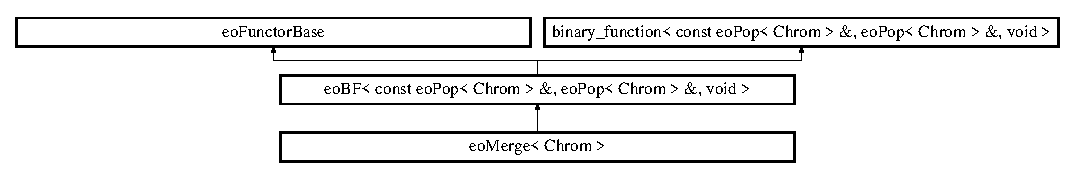
\includegraphics[height=1.94896cm]{classeo_merge}
\end{center}
\end{figure}


\subsection{Detailed Description}
\subsubsection*{template$<$class Chrom$>$ class eo\-Merge$<$ Chrom $>$}

eo\-Merge: Base class for elitist replacement algorithms. 

Merges the old population (first argument), with the new generation

Its signature is exactly that of the selection base {\bf eo\-Select}{\rm (p.\,\pageref{classeo_select})}, but its purpose is to merge the two populations into one (the second argument). Note that the algorithms assume that the second argument denotes the next generation. 



Definition at line 48 of file eo\-Merge.h.

The documentation for this class was generated from the following file:\begin{CompactItemize}
\item 
eo\-Merge.h\end{CompactItemize}
